\clearpage
\section{Pembahasan dan Implementasi}
\subsection{Struktur Repositori dan Antarmuka Model}
Repositori \texttt{IF3170\_G02\_nutellabear} memisahkan kode kelas dari notebook pengumpulan. Kelas model dan modul pendukung berada di \path{src/}, lalu di-\textit{import} atau disalin ke notebook templat asisten agar notebook dapat dijalankan pula di Kaggle. Hasil \textit{run} disimpan di \path{output/}, laporan di \path{docs/}, dan pengujian unit di \path{tests/}.

\begin{lstlisting}[language={},caption={Struktur repositori},label={lst:struktur}]
.
|-- T2-IF3170-2026-2027/   train.csv, test.csv, sample_submission.csv
|-- nb/                    notebook templat pengumpulan
|-- src/
|   |-- preprocessing.py   split, cleaning, langkah persiapan, pipeline
|   |-- evaluation.py      metrik, ROC-AUC, stratified k-fold, cross_validate
|   |-- knn.py, decision_tree.py, logreg.py, svm.py, naive_bayes.py
|   |-- knn_tuning.py, dtl_tuning.py     eksperimen optimasi model
|   |-- cost_sensitive.py, nb_graph.py, nb_compare.py, eda.py
|   |-- submission.py      make_submission, check_reproducible
|-- tests/                 pengujian unit per modul (pytest)
|-- output/                gambar, video, dan CSV submission
|-- docs/                  laporan
\end{lstlisting}

Kelima model memakai antarmuka yang seragam: \texttt{fit(X, y)}, \texttt{predict\_proba(X)} yang mengembalikan peluang kelas 1 berbentuk $(m,)$, \texttt{predict(X, threshold=0.5)}, \texttt{save(path)}, dan \texttt{load(path)}. Dengan antarmuka ini, modul evaluasi, validasi silang, \textit{cost-sensitive}, dan \textit{submission} dapat memanggil setiap model dengan cara yang sama. Implementasi \textit{from scratch} hanya memakai NumPy untuk perhitungan. Pustaka \textit{scikit-learn} dipakai untuk pembagian data, \textit{mutual information}, PCA, dan model pembanding.

\begin{figure}[htbp]
    \centering
    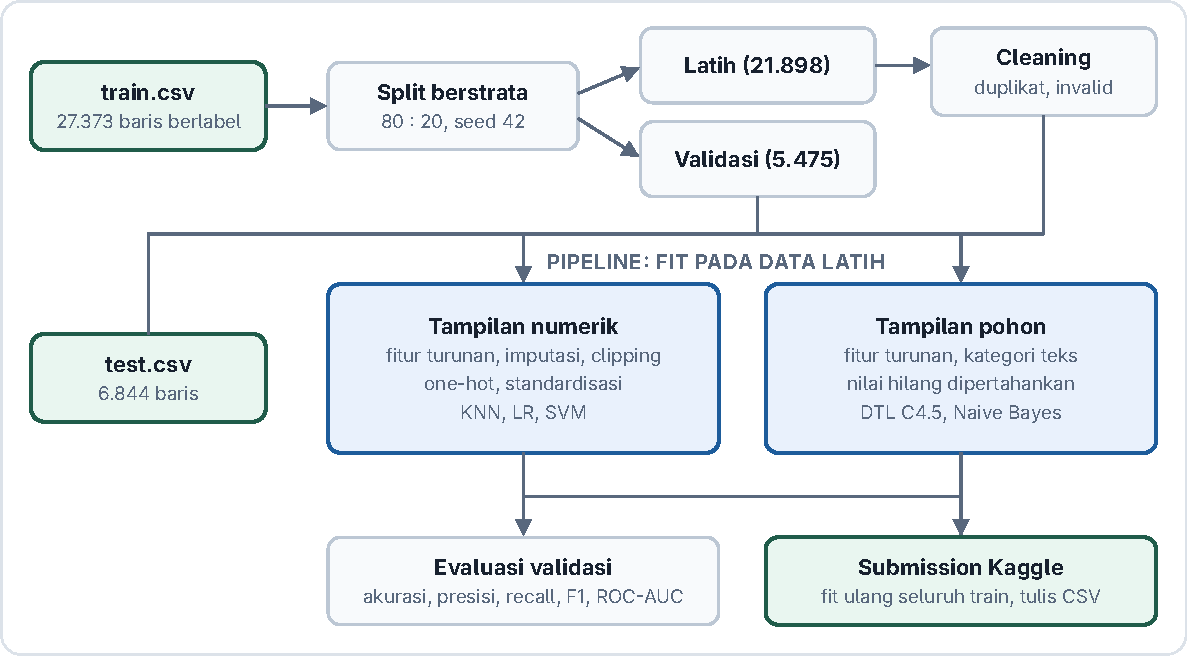
\includegraphics[width=\textwidth]{diagram/pipeline.pdf}
    \caption{Alur pengolahan data dari pembagian hingga evaluasi dan \textit{submission}.}
    \label{fig:pipeline}
\end{figure}

\subsection{\textit{Data Cleaning} dan \textit{Preprocessing}}\label{sec:preprocessing}
Gambar~\ref{fig:pipeline} merangkum alur pengolahan data. Seluruh langkah yang mempelajari statistik dari data dibungkus dalam kelas dengan metode \texttt{fit} dan \texttt{transform}, lalu dirangkai oleh \texttt{PreparationPipeline}. Pipeline di-\textit{fit} hanya pada data latih, sedangkan data validasi dan uji hanya di-\textit{transform}, sehingga tidak terjadi \textit{data leakage}.

\begin{lstlisting}[emph={PreparationPipeline,numeric_pipeline,tree_pipeline},caption={Pipeline dan dua tampilan data (\texttt{src/preprocessing.py})},label={lst:pipeline}]
class PreparationPipeline:
    def _run(self, df, fit):
        df = df.drop(columns=[ID_COL], errors="ignore")
        for step in self.steps:
            if callable(step):  # fungsi tanpa state, mis. construct_features
                df = step(df)
            else:
                df = (step.fit(df) if fit else step).transform(df)
        return df

def numeric_pipeline(select_k=None, pca=None):
    """Tampilan numerik (KNN, LR, SVM): tanpa NaN, one-hot, terskala."""
    steps = [construct_features, Imputer(), Clipper(), CategoricalEncoder(), Scaler()]
    ...

def tree_pipeline(impute=False):
    """Tampilan pohon (DTL, NB): kategori tetap teks, NaN dibiarkan."""
    return PreparationPipeline([construct_features] + ([Imputer()] if impute else []))
\end{lstlisting}

\subsubsection{Pembagian Data}
\texttt{split\_train\_val} membagi \path{train.csv} menjadi 80\% data latih (21.898 baris) dan 20\% data validasi (5.475 baris) secara berstrata terhadap \texttt{is\_canceled} dengan \texttt{seed=42}. Proporsi kelas batal pada kedua bagian sama, yaitu 32,77\%. Seluruh anggota memakai pembagian dan \textit{seed} yang sama agar angka antarmodel dapat dibandingkan. Validasi silang lima lipatan memakai fungsi \texttt{stratified\_kfold} buatan sendiri dengan \textit{seed} yang sama.

\subsubsection{Duplikat dan Data Tidak Valid}
\texttt{drop\_duplicates\_and\_invalid} hanya diterapkan pada data latih. Kelompok baris dengan fitur identik tetapi label berbeda dibuang seluruhnya, karena tidak ada cara menentukan label yang benar dan keberadaannya hanya menambah derau. Kelompok duplikat lain disisakan satu baris agar pola yang sama tidak berbobot ganda. Baris dengan nilai negatif atau tanpa tamu sama sekali dianggap mustahil dan dibuang. Pada data latih hasil pembagian, langkah ini membuang 2 baris berlabel konflik dan 40 duplikat, sehingga tersisa 21.856 baris.

Beberapa nilai yang tampak janggal sengaja dipertahankan karena mengandung informasi tentang pembatalan. Tabel~\ref{tab:nilai-janggal} menunjukkan bahwa pemesanan tanpa malam menginap dan pemesanan bertarif nol hampir tidak pernah batal. Kemungkinan besar keduanya mewakili pemesanan khusus, seperti \textit{day use} atau kamar gratis, sehingga membuangnya justru menghapus pola yang berguna. Data validasi dan uji tidak dibersihkan karena setiap barisnya tetap harus memperoleh prediksi.

\begin{table}[htbp]
    \centering
    \small
    \begin{tabular}{@{}l r r@{}}
        \toprule
        Kondisi pada data latih & Jumlah baris & Rasio batal \\
        \midrule
        Tanpa malam menginap & 49 & 0,0408 \\
        Tanpa tamu dewasa & 84 & 0,2976 \\
        Tarif per malam nol & 324 & 0,0062 \\
        Tanpa tamu sama sekali / nilai negatif & 0 & -- \\
        \bottomrule
    \end{tabular}
    \caption{Nilai janggal pada data latih beserta rasio pembatalannya.}
    \label{tab:nilai-janggal}
\end{table}

\subsubsection{Nilai Hilang}
Tampilan numerik mengisi nilai hilang dengan median untuk fitur numerik dan modus untuk fitur kategorikal. Median dipilih karena beberapa fitur, seperti tarif dan \texttt{days\_before\_arrival}, memiliki distribusi miring dengan pencilan. Nilai pengisi yang dipelajari dari data latih antara lain 57 hari untuk \texttt{days\_before\_arrival}, Rp1.647.000 untuk \texttt{nightly\_rate\_idr}, Breakfast untuk \texttt{meal\_package}, dan Type B untuk \texttt{room\_category}.

Untuk \texttt{special\_requests}, \texttt{Imputer} juga menambahkan kolom indikator \texttt{special\_requests\_missing}. Alasannya, rasio batal baris yang nilai ini hilang mencapai 0,4074, jauh di atas 0,3196 pada baris yang nilainya ada. Pola hilangnya data ini sendiri informatif, sehingga indikator mempertahankan informasi yang akan hilang bila nilai hanya diisi median. Fitur lain tidak menunjukkan perbedaan sebesar itu.

Tampilan pohon tidak mengimputasi nilai hilang. DTL C4.5 menangani nilai hilang dengan bobot pecahan, sedangkan \textit{Naive Bayes} cukup melewati fitur yang hilang ketika menghitung \textit{likelihood}. Dengan cara ini kedua model tidak bergantung pada nilai tebakan.

\subsubsection{Pencilan}
\texttt{Clipper} memotong \texttt{days\_before\_arrival}, \texttt{nightly\_rate\_idr}, dan \texttt{nightly\_rate\_per\_guest} ke persentil 1\% dan 99\% data latih. Ketiga fitur tersebut kontinu dan memiliki ekor panjang, sehingga nilai ekstremnya dapat mendominasi jarak KNN, kernel SVM, dan gradien \textit{logistic regression}. Batas atas yang dipelajari adalah 342 hari dan Rp3.408.000, dan sekitar 218 baris latih terpotong pada setiap fitur. Fitur hitungan seperti \texttt{prior\_cancellations} tidak dipotong karena persentil 99\%-nya bernilai 0. Pemotongan akan menghapus informasi penting karena 183 baris dengan \texttt{prior\_cancellations} positif hanya memiliki rasio batal 0,044, jauh di bawah 0,330 pada baris lain.

\subsubsection{Konstruksi Fitur}
\texttt{construct\_features} menambahkan tiga fitur turunan: \texttt{total\_nights} (jumlah malam akhir pekan dan hari kerja), \texttt{total\_guests} (jumlah tamu dewasa dan anak), serta \texttt{nightly\_rate\_per\_guest} (tarif dibagi jumlah tamu). Fitur-fitur ini merangkum besar pemesanan dan harga per orang, yang secara intuitif berkaitan dengan komitmen tamu. Korelasi Spearman ketiganya terhadap target berturut-turut 0,089, 0,081, dan 0,035, sehingga hubungannya dengan target ada tetapi lemah. Fitur turunan dipakai pada tampilan numerik dan tampilan pohon. Konfigurasi \textit{Naive Bayes} memakai fitur asli karena validasi silang menunjukkan fitur turunan menurunkan akurasinya (Subbab~\ref{sec:hasil-nb}).

\subsubsection{\textit{Encoding} dan Penskalaan}
\texttt{CategoricalEncoder} melakukan \textit{one-hot encoding} dengan daftar kategori dari data latih: 4 kategori \texttt{meal\_package}, 7 kategori \texttt{room\_category}, dan 5 kategori \texttt{booking\_channel}. Kategori yang tidak dikenal pada data baru dikodekan sebagai vektor nol sehingga tidak menimbulkan galat. \textit{One-hot} dipilih karena ketiga fitur bersifat nominal. Pengodean ordinal akan memaksakan urutan yang sebenarnya tidak ada sehingga memengaruhi jarak serta bobot linear.

\texttt{Scaler} melakukan standardisasi dengan rata-rata dan simpangan baku data latih. Kolom konstan diberi skala 1 untuk menghindari pembagian dengan nol. Setelah transformasi, rata-rata fitur pada data validasi mendekati 0 dan simpangan bakunya mendekati 1. Hasil akhir tampilan numerik adalah 34 kolom tanpa nilai hilang. Tampilan pohon berisi 20 kolom dengan kategori asli dan 17.990 sel bernilai hilang pada data latih.

\subsubsection{Seleksi Fitur, Reduksi Dimensi, dan Ketidakseimbangan Kelas}
Ketiga teknik ini diimplementasikan sebagai langkah opsional dan diuji pada KNN, karena KNN paling peka terhadap fitur yang tidak relevan dan dimensi tinggi. \texttt{FeatureSelector} memilih $k$ fitur dengan \textit{mutual information} tertinggi terhadap target. Fitur paling informatif adalah \texttt{days\_before\_arrival} (0,1020), \texttt{special\_requests} (0,0376), dan \texttt{nightly\_rate\_idr} (0,0268). \texttt{DimReducer} menerapkan PCA dan membutuhkan 25 dari 34 komponen untuk melampaui 95\% ragam kumulatif. Karena ragam tersebar pada banyak komponen, PCA tidak banyak memampatkan data ini. \texttt{handle\_imbalance} melakukan \textit{random oversampling} kelas minoritas dari 7.161 menjadi 14.695 baris, hanya pada data latih. Hasil ketiga variasi dibahas pada Subbab~\ref{sec:hasil-knn}. Pipeline baku tidak memakainya.

\subsection{Implementasi \textit{k-Nearest Neighbors}}
Kelas \texttt{KNN} pada \path{src/knn.py} menyimpan salinan data latih pada \texttt{fit}. Matriks jarak dihitung secara tervektorisasi per \textit{batch} 256 baris kueri agar memori tetap aman. Matriks penuh $5.475\times21.856$ bertipe \textit{float64} akan memerlukan sekitar 1 GB. Untuk jarak Euclidean, identitas $\|\mathbf{a}-\mathbf{b}\|^2=\|\mathbf{a}\|^2+\|\mathbf{b}\|^2-2\mathbf{a}^\top\mathbf{b}$ memungkinkan perhitungan dengan satu perkalian matriks. Untuk orde Minkowski lain, selisih diakumulasi per fitur agar tidak terbentuk larik tiga dimensi.

\begin{lstlisting}[emph={_pairwise_distances,kneighbors},caption={Perhitungan jarak dan pencarian tetangga (\texttt{src/knn.py})},label={lst:knn}]
def _pairwise_distances(self, Xq):
    p = {"euclidean": 2, "manhattan": 1}.get(self.metric, self.p)
    if p == 2:  # ||a-b||^2 = ||a||^2 + ||b||^2 - 2ab
        sq = (Xq ** 2).sum(1)[:, None] + (self.X_ ** 2).sum(1)[None, :] - 2 * Xq @ self.X_.T
        return np.sqrt(np.maximum(sq, 0))
    D = np.zeros((len(Xq), len(self.X_)))
    for j in range(Xq.shape[1]):  # per fitur, hindari array 3D
        D += np.abs(Xq[:, j, None] - self.X_[None, :, j]) ** p
    return D if p == 1 else D ** (1 / p)

def kneighbors(self, X):
    for s in range(0, len(X), self.batch_size):
        D = self._pairwise_distances(X[s:s + self.batch_size])
        nn = np.argpartition(D, self.k - 1, axis=1)[:, :self.k]  # k terkecil
        ...
\end{lstlisting}

Pemilihan $k$ tetangga memakai \texttt{np.argpartition} yang berjalan dalam waktu linear, lalu hanya $k$ jarak terpilih yang diurutkan. \texttt{predict\_proba} mengikuti Persamaan~\ref{eq:knn-proba}. Pada pembobotan \textit{distance}, bila ada tetangga berjarak nol, hanya titik identik tersebut yang dihitung, sesuai perilaku \textit{scikit-learn}.

\subsection{Implementasi \textit{Decision Tree Learning} (C4.5)}
Kelompok memilih C4.5 karena varian ini secara alami menangani atribut numerik, atribut kategorikal, dan nilai hilang, sesuai kebutuhan dataset ini. Kelas \texttt{DecisionTree} pada \path{src/decision_tree.py} menyimpan simpul sebagai \texttt{TreeNode} berisi jumlah kelas berbobot, fitur pemisah, ambang atau kategori, anak, dan peluang cabang untuk nilai hilang.

Untuk atribut numerik, \texttt{\_best\_numeric} mengurutkan nilai yang diketahui, lalu menghitung jumlah kelas kumulatif sehingga seluruh kandidat ambang dievaluasi sekaligus dalam $O(n\log n)$. \textit{Gain} pada sampel diketahui dikalikan proporsi bobot yang diketahui, dan nilai hilang diperlakukan sebagai partisi tambahan pada \textit{split information}, sesuai Subbab dasar teori.

\begin{lstlisting}[emph={_best_numeric},caption={Evaluasi seluruh ambang numerik secara kumulatif (\texttt{src/decision\_tree.py}, diringkas)},label={lst:dtl-numeric}]
positions = np.flatnonzero(values[:-1] < values[1:])  # batas antar nilai berbeda
cumulative, positive = np.cumsum(w), np.cumsum(w * labels)
left_w, left_pos = cumulative[positions], positive[positions]
right_w, right_pos = cumulative[-1] - left_w, positive[-1] - left_pos
known_w, missing_w = cumulative[-1], weights[~known].sum()
gain = np.maximum(0.0, known_w / (known_w + missing_w) *
                  (parent_h - (left_w * _entropy_counts(left)
                               + right_w * _entropy_counts(right)) / known_w))
split_info = _entropy_counts(np.column_stack((masses, np.full(len(masses), missing_w))))
ratios = np.divide(gain, split_info, out=np.zeros_like(gain), where=split_info > 1e-12)
\end{lstlisting}

Atribut kategorikal dipecah per kategori (\textit{multiway}) dan tidak diuji ulang pada keturunannya. Pemilihan atribut mengikuti aturan C4.5: hanya kandidat dengan \textit{gain} minimal sebesar rata-rata yang dibandingkan \textit{gain ratio}-nya.

\begin{lstlisting}[caption={Pemilihan split dan pembagian bobot pecahan (\texttt{src/decision\_tree.py}, diringkas)},label={lst:dtl-split}]
average_gain = np.mean([s.gain for s in candidates])
eligible = [s for s in candidates if s.gain >= average_gain - 1e-12]
split = max(eligible, key=lambda s: s.ratio)
...
for branch, key in enumerate(keys):
    probability = float(split.probabilities[branch])
    mask = (branches == branch) | missing          # sampel hilang ikut ke semua cabang
    child_w = w[mask] * np.where(missing[mask], probability, 1.0)
\end{lstlisting}

Pohon dibangun secara iteratif dengan \textit{stack}, bukan rekursi, sehingga tidak ada risiko melampaui batas rekursi Python pada data besar. Pertumbuhan berhenti apabila simpul murni, jumlah sampel kurang dari \texttt{min\_samples\_split}, kedalaman mencapai \texttt{max\_depth} (baku 20), atau tidak ada kandidat dengan \textit{gain} melebihi \texttt{min\_gain}. Pada prediksi, sampel dengan nilai hilang atau kategori baru menelusuri seluruh cabang, dan peluang daun digabung menurut bobot cabang.

\subsection{Implementasi \textit{Logistic Regression}}
Kelas \texttt{LogisticRegression} pada \path{src/logreg.py} meminimalkan rata-rata \textit{log-loss} ditambah penalti (Persamaan~\ref{eq:logloss} dan~\ref{eq:reg}). Fungsi sigmoid ditulis stabil secara numerik dengan memisahkan kasus $z\geq0$ dan $z<0$, sehingga tidak terjadi \textit{overflow} untuk $|z|$ besar. Regularisasi dirancang sebagai hierarki kelas \texttt{Regularizer} dengan subkelas \texttt{L1}, \texttt{L2}, dan \texttt{ElasticNet}. Setiap subkelas menyediakan gradien bagian mulus (\texttt{grad\_smooth}) dan operator proksimal bagian L1 (\texttt{prox}).

\begin{lstlisting}[emph={ElasticNet,_soft_threshold},caption={Regularizer Elastic Net dengan langkah proksimal (\texttt{src/logreg.py})},label={lst:lr-reg}]
def _soft_threshold(w, t):
    return np.sign(w) * np.maximum(np.abs(w) - t, 0.0)

class ElasticNet(Regularizer):
    def grad_smooth(self, w):
        return self.alpha * (1 - self.l1_ratio) * w
    def prox(self, w, step):
        return _soft_threshold(w, step * self.alpha * self.l1_ratio)
\end{lstlisting}

Setiap iterasi melakukan langkah gradien pada \textit{log-loss} dan bagian L2, lalu menerapkan \textit{soft-threshold} untuk bagian L1. Dengan cara ini, bobot fitur yang tidak berguna menjadi tepat nol, bukan hanya mendekati nol. Bias tidak diregularisasi. Pelatihan berhenti apabila perubahan objektif antar-\textit{epoch} lebih kecil dari \texttt{tol}, dan riwayat objektif serta parameter disimpan pada \texttt{history\_} untuk keperluan video lintasan parameter.

\begin{lstlisting}[caption={Langkah pembaruan \textit{gradient descent} proksimal (\texttt{src/logreg.py}, diringkas)},label={lst:lr-fit}]
err = sigmoid(X[idx] @ w + b) - y[idx]
grad_w = X[idx].T @ err / len(idx) + reg.grad_smooth(w)
grad_b = err.mean()
w = reg.prox(w - self.lr * grad_w, self.lr)   # soft-threshold untuk bagian L1
b -= self.lr * grad_b
\end{lstlisting}

Optimizer tambahan ditempatkan pada subkelas \texttt{OptimizedLogisticRegression} di \path{src/logreg_optim.py} agar kelas induk tidak berubah. Subkelas ini menyediakan \texttt{optimizer="fista"} dan \texttt{optimizer="adam"}. Pada FISTA, laju belajar baku adalah $1/L$, dengan $\lambda_{\max}$ dihitung melalui iterasi pangkat pada matriks data yang diberi kolom satu untuk bias.

\begin{lstlisting}[caption={Satu iterasi FISTA (\texttt{src/logreg\_optim.py}, diringkas)},label={lst:fista}]
t_next = (1 + np.sqrt(1 + 4 * momentum_t ** 2)) / 2
z = theta + (momentum_t - 1) / t_next * (theta - previous)   # titik ekstrapolasi
g = gradient(z, np.arange(n))
new = z - self.lr * g
new[1:] = reg.prox(new[1:], self.lr)                          # bias tidak diregularisasi
previous, theta, momentum_t = theta, new, t_next
\end{lstlisting}

Konfigurasi baku memakai \textit{batch} penuh, laju belajar 0,1, $\alpha=0{,}01$, dan \texttt{l1\_ratio}=0,5. Hubungan dengan \textit{scikit-learn} adalah $\alpha=1/(C\,n)$, karena \textit{scikit-learn} meminimalkan $C\sum_i\ell_i+R(\mathbf{w})$. Hubungan ini dipakai agar kedua implementasi membandingkan fungsi tujuan yang sama.

\subsection{Implementasi \textit{Support Vector Machine}}
Kelas \texttt{SVM} pada \path{src/svm.py} menyelesaikan bentuk dual (Persamaan~\ref{eq:svm-dual}) dengan SMO. Setiap kernel adalah kelas dengan metode \texttt{compute(A, B)} yang mengembalikan matriks kernel secara tervektorisasi. Nilai baku $\gamma$ untuk kernel polinomial dan Gaussian adalah $1/m$ dengan $m$ jumlah fitur, sesuai opsi \texttt{gamma='auto'} pada \textit{scikit-learn}.

\begin{lstlisting}[emph={_smo},caption={Iterasi SMO dengan pemilihan \textit{maximal violating pair} (\texttt{src/svm.py})},label={lst:smo}]
for it in range(self.max_iter):
    up  = ((y > 0) & (alpha < C)) | ((y < 0) & (alpha > 0))
    low = ((y > 0) & (alpha > 0)) | ((y < 0) & (alpha < C))
    score = -y * G
    i = np.flatnonzero(up)[np.argmax(score[up])]
    j = np.flatnonzero(low)[np.argmin(score[low])]
    gap = score[i] - score[j]
    if gap < self.tol:          # KKT terpenuhi dalam toleransi
        self.converged_ = True
        break
    eta = max(diagK[i] + diagK[j] - 2 * K[i, j], 1e-12)
    t = min(gap / eta,
            C - alpha[i] if y[i] > 0 else alpha[i],
            alpha[j] if y[j] > 0 else C - alpha[j])
    alpha[i] += y[i] * t
    alpha[j] -= y[j] * t
    G += y * t * (K[:, i] - K[:, j])
\end{lstlisting}

Vektor $G$ menyimpan gradien objektif dual dan diperbarui secara inkremental hanya dengan dua kolom matriks kernel, sehingga setiap iterasi berjalan dalam $O(n)$. Setelah konvergen, bias $b$ dihitung dari rata-rata \textit{support vector} bebas ($0<\alpha_i<C$), dan hanya sampel dengan $\alpha_i>10^{-8}$ yang disimpan sebagai \textit{support vector}.

Strategi skala data menjadi keputusan desain terpenting pada SVM. Matriks kernel penuh untuk 21.856 baris latih memerlukan sekitar 3,8 GB dalam presisi ganda. Karena itu, apabila jumlah data melebihi \texttt{max\_samples}, SVM dilatih pada subsampel berstrata (baku 4.000 baris) dengan matriks kernel penuh di-\textit{cache}. Hingga 5.000 baris di luar subsampel dipakai untuk \textit{Platt scaling}, sehingga kalibrasi peluang tidak dilakukan pada data yang sama dengan pelatihan SVM. Parameter Platt dicari dengan metode Newton dan target ter-\textit{smoothing} menurut Lin dkk.. Subkelas \texttt{SVMWSS2} pada \path{src/svm_wss.py} hanya mengganti pemilihan indeks $j$ pada SMO dengan kriteria orde kedua. Kandidat $j$ dibatasi pada $I_{\mathrm{low}}$ dengan skor lebih kecil daripada skor $i$, lalu dipilih yang meminimalkan $-b_{ij}^2/a_{ij}$, dengan $a_{ij}$ diganti $10^{-12}$ bila tidak positif. Kriteria berhenti dan perhitungan bias sama dengan kelas induk.

\subsection{Implementasi \textit{Naive Bayes}}
Kelas \texttt{NaiveBayes} pada \path{src/naive_bayes.py} menerima tampilan data dengan kategori asli. Fitur numerik dengan lebih dari sepuluh nilai unik didiskretisasi, sedangkan fitur lain diperlakukan sebagai kategori. Parameter \texttt{discretization} memilih cara diskretisasi. Nilai baku \texttt{"quantile"} memakai 20 interval kuantil, sedangkan \texttt{"mdl"} memakai ambang Fayyad--Irani yang dihitung dari label data latih dengan nilai hilang diabaikan. Setiap fitur memiliki satu tingkat tambahan untuk kategori yang tidak dikenal pada data latih, sehingga data baru tidak menimbulkan galat.

\begin{lstlisting}[emph={fit,predict_proba},caption={Estimasi \textit{likelihood} dengan Laplace smoothing dan normalisasi \textit{log-sum-exp} (\texttt{src/naive\_bayes.py}, diringkas)},label={lst:nb}]
n_class = np.bincount(y, minlength=2)
self.log_prior_ = np.log((n_class + self.alpha) / (len(y) + 2 * self.alpha))
for c in self.columns_:
    codes = self._codes(c, col)              # -1 untuk nilai hilang
    counts = np.zeros((2, n_levels + 1))
    for k in (0, 1):
        seen = codes[(y == k) & (codes >= 0)]
        counts[k] = np.bincount(seen, minlength=n_levels + 1)
    self.log_lik_[c] = np.log((counts + self.alpha) /
                              (counts.sum(1, keepdims=True) + self.alpha * (n_levels + 1)))

# predict_proba
score = np.tile(self.log_prior_, (len(X), 1))
for c in self.columns_:
    codes = self._codes(c, X[c]); known = codes >= 0
    score[known] += self.log_lik_[c][:, codes[known]].T   # fitur hilang dilewati
peak = score.max(axis=1, keepdims=True)
log_norm = peak + np.log(np.exp(score - peak).sum(axis=1, keepdims=True))
return np.exp(score - log_norm)[:, 1]
\end{lstlisting}

Perhitungan dilakukan dalam ruang log, dan fitur yang nilainya hilang tidak menyumbang \textit{likelihood}. Pendekatan ini setara dengan marginalisasi fitur tersebut, karena $\sum_v P(x_j=v\mid C)=1$. Normalisasi \textit{log-sum-exp} mencegah \textit{underflow}, dan jumlah peluang kedua kelas selalu satu.

\subsection{Evaluasi, Penyimpanan Model, dan \textit{Submission}}
Modul \path{src/evaluation.py} mengimplementasikan \textit{confusion matrix}, akurasi, presisi, \textit{recall}, F1, dan ROC-AUC. ROC-AUC dihitung sebagai statistik Mann--Whitney dengan rata-rata peringkat untuk skor kembar. Fungsi \texttt{cross\_validate} menerima fungsi \texttt{prepare(train\_df, val\_df)} yang dipanggil pada setiap lipatan, sehingga pipeline di-\textit{fit} ulang pada bagian latih lipatan tersebut.

Model disimpan dengan \texttt{pickle}, kecuali \texttt{WeightedKNN} yang memakai format \texttt{.npz} tanpa \textit{pickle}. Notebook menyimpan lima konfigurasi pengumpulan serta eksperimen SVM Gaussian 12.000 baris, memuat ulang masing-masing, lalu memastikan peluang hasil muat ulang cocok dalam toleransi $10^{-12}$ dan label prediksinya identik. Keenam pemeriksaan lolos.

Fungsi \texttt{make\_submission} membersihkan seluruh \path{train.csv}, melatih ulang pipeline dan model pada data tersebut, lalu hanya men-\textit{transform} \path{test.csv}. Keluarannya adalah CSV berisi \texttt{id} dan \texttt{is\_canceled} dengan 6.844 baris, sama dengan format \path{sample_submission.csv}. Fungsi \texttt{check\_reproducible} membandingkan dua berkas \textit{submission} tanpa memperhatikan urutan baris.
